\hypertarget{digital-signal-processing-dsp---session-6}{%
\section{Digital Signal Processing (DSP) - Session
6}\label{digital-signal-processing-dsp---session-6}}

\begin{center}\rule{0.5\linewidth}{0.5pt}\end{center}

\hypertarget{the-discrete-fourier-transform}{%
\subsection{The Discrete Fourier
Transform}\label{the-discrete-fourier-transform}}

The objective of the Discrete Fourier Transform (DFT) is to provide a
\textbf{computationally convenient frequency-domain representation} of a
discrete-time sequence.

Because the standard Fourier transform of an aperiodic sequence is a
continuous function of frequency, it cannot be processed directly by
digital hardware. The DFT solves this by \textbf{representing the
sequence through samples of its spectrum}, making it a powerful tool for
performing \textbf{frequency analysis} on digital signal processors and
computers.

\hypertarget{frequency-domain-sampling-and-reconstruction-of-discrete-time-signals}{%
\subsubsection{Frequency-Domain Sampling and Reconstruction of
Discrete-Time
Signals}\label{frequency-domain-sampling-and-reconstruction-of-discrete-time-signals}}

\begin{itemize}
\tightlist
\item
  \textbf{Objective of Sampling:} To perform frequency analysis on a
  digital processor, the continuous Fourier transform \(X(\omega)\) must
  be represented by a discrete set of frequency samples. This process
  leads to the \textbf{Discrete Fourier Transform (DFT)}.
\item
  \textbf{Sampling Strategy:} We take \(N\) equidistant samples in the
  interval \(0 \leq \omega < 2\pi\) with a spacing of
  \(\delta \omega = 2\pi/N\).

  \begin{itemize}
  \tightlist
  \item
    While real signals have symmetric spectra allowing characterization
    within the range \([0, \pi]\), the standard DFT derivation utilizes
    the full \(2\pi\) period.
  \end{itemize}
\item
  \textbf{Time-Domain Impact (Periodic Extension):} Sampling the
  spectrum in the frequency domain results in a \textbf{periodic
  extension} of the original time-domain sequence \(x(n)\). The
  resulting periodic signal \(x_p(n)\) is defined as:
  \[x_p(n) = \sum_{l=-\infty}^{\infty} x(n-lN)\]
\item
  \textbf{Information Preservation \& Aliasing:} To recover the original
  sequence \(x(n)\) from the periodic version \(x_p(n)\), we must avoid
  \textbf{time-domain aliasing}.

  \begin{itemize}
  \tightlist
  \item
    This is possible only if \(x(n)\) is finite-duration with length
    \(L\).
  \item
    The number of frequency samples must satisfy \textbf{\(N \ge L\)} to
    ensure that \(x(n) = x_p(n)\) for \(0 \leq n \leq N-1\).
  \item
    If \(N < L\), the cycles of the periodic extension overlap, causing
    aliasing and loss of information.
  \end{itemize}
\item
  \textbf{Consequence for Infinite Signals:} If the signal length
  \(L \rightarrow \infty\), then the number of samples \(N\) must also
  approach \(\infty\) to avoid aliasing. This means infinite
  frequency-domain samples are required to represent an
  infinite-duration aperiodic signal.
\item
  \textbf{Reconstruction Formula:} If \(N \ge L\), the continuous
  spectrum \(X(\omega)\) can be reconstructed from its discrete samples
  \(X(\frac{2\pi}{N}k)\) using the following interpolation formula:
  \[X(\omega) = \sum_{k=0}^{N-1} X\left(\frac{2\pi}{N}k\right) P\left(\omega - \frac{2\pi}{N}k\right)\]
  where the interpolation function \(P(\omega)\) is defined as:
  \[P(\omega) = \frac{\sin(\omega N/2)}{N \sin(\omega/2)} e^{-j\omega(N-1)/2}\]
\end{itemize}

\begin{quote}
\textbf{\emph{Example 1.1}}

Consider the signal \[x(n) = a^n u(n), \quad 0 < a < 1\] The spectrum of
this signal is sampled at \(N\) equidistant frequencies
\(\omega_k = 2\pi k/N\) for \(k = 0, 1, \dots, N-1\). Determine the
reconstructed spectra for \(a = 0.8\) when \(N = 5\) and \(N = 50\).

\emph{Solution}

\textbf{1. Determine the Fourier Transform of the Signal:} The Fourier
transform of the infinite-duration sequence \(x(n)\) is:
\[X(\omega) = \sum_{n=0}^{\infty} a^n e^{-j\omega n} = \frac{1}{1 - ae^{-j\omega}}\]

\textbf{2. Evaluate Spectral Samples:} Sampling \(X(\omega)\) at \(N\)
equidistant frequencies yields:
\[X(k) \equiv X\left(\frac{2\pi k}{N}\right) = \frac{1}{1 - ae^{-j2\pi k/N}}, \quad k = 0, 1, \dots, N-1\]

\textbf{3. Identify the Corresponding Time-Domain Periodic Sequence:}
The frequency samples \(X(k)\) correspond to the periodic extension of
\(x(n)\), defined as \(x_p(n) = \sum_{l=-\infty}^{\infty} x(n-lN)\). For
this signal:
\[x_p(n) = \sum_{l=-\infty}^{0} a^{n-lN} = a^n \sum_{l=0}^{\infty} a^{lN}\]
Evaluating the geometric series:
\[x_p(n) = \frac{a^n}{1 - a^N}, \quad 0 \le n \le N-1\]

\textbf{4. Analyze the Effect of Aliasing:} The factor
\(\frac{1}{1 - a^N}\) represents the \textbf{effect of time-domain
aliasing}.

\begin{itemize}
\tightlist
\item
  As \(N \rightarrow \infty\), the factor approaches 1, meaning aliasing
  becomes negligible.
\item
  For \textbf{\(N = 5\) and \(a = 0.8\)}, \(1 - a^N \approx 0.672\),
  resulting in a significant aliasing error.
\item
  For \textbf{\(N = 50\) and \(a = 0.8\)}, \(1 - a^N \approx 1\),
  meaning aliasing is virtually nonexistent.
\end{itemize}

\textbf{5. Determine the Reconstructed Spectrum:} The Fourier transform
\(\hat{X}(\omega)\) of the aliased finite-duration sequence
\(\hat{x}(n)\) (where \(\hat{x}(n) = x_p(n)\) for \(0 \le n \le N-1\))
is:
\[\hat{X}(\omega) = \sum_{n=0}^{N-1} x_p(n) e^{-j\omega n} = \frac{1}{1 - a^N} \cdot \frac{1 - a^N e^{-j\omega N}}{1 - ae^{-j\omega}}\]

\textbf{6. Conclusion:} While \(\hat{X}(\omega) \neq X(\omega)\), they
are \textbf{identical at the sample points} \(\omega_k = 2\pi k/N\).
When \(N=5\), the reconstructed spectrum is a poor approximation due to
aliasing; when \(N=50\), it closely matches the original continuous
spectrum.
\end{quote}

\hypertarget{the-discrete-fourier-transform-dft}{%
\subsubsection{The Discrete Fourier Transform
(DFT)}\label{the-discrete-fourier-transform-dft}}

The DFT provides a \textbf{computationally convenient frequency-domain
representation} for discrete-time sequences, allowing frequency analysis
to be performed on digital hardware.

\hypertarget{mathematical-definition}{%
\paragraph{Mathematical Definition}\label{mathematical-definition}}

The DFT maps a sequence \(x(n)\) of length \(L\) into a sequence of
frequency samples \(X(k)\) of length \(N\), where \(N \ge L\).

\begin{itemize}
\tightlist
\item
  \textbf{DFT (Analysis Equation):}
  \[X(k) = \sum_{n=0}^{N-1} x(n)e^{-j2\pi kn/N}, \quad k = 0, 1, \dots, N-1 \quad\]
\item
  \textbf{IDFT (Synthesis Equation):}
  \[x(n) = \frac{1}{N} \sum_{k=0}^{N-1} X(k)e^{j2\pi kn/N}, \quad n = 0, 1, \dots, N-1 \quad\]
\end{itemize}

\hypertarget{derivation-and-frequency-sampling}{%
\paragraph{Derivation and Frequency
Sampling}\label{derivation-and-frequency-sampling}}

The DFT is derived by \textbf{sampling the continuous Fourier transform}
\(X(\omega)\) at \(N\) equidistant frequencies
\(\omega_k = \frac{2\pi k}{N}\).

\begin{itemize}
\tightlist
\item
  \textbf{Time-Domain Impact:} Sampling in frequency results in a
  \textbf{periodic extension} of the original signal:
  \[x_p(n) = \sum_{l=-\infty}^{\infty} x(n-lN)\]
\item
  \textbf{Aliasing Condition:} To recover the original sequence \(x(n)\)
  from these samples, the number of samples \(N\) must satisfy
  \textbf{\(N \ge L\)} to avoid \textbf{time-domain aliasing}.
\item
  \textbf{Reconstruction:} If \(N \ge L\), the continuous spectrum
  \(X(\omega)\) can be reconstructed from the DFT samples \(X(k)\) using
  an \textbf{interpolation formula}.
\end{itemize}

\hypertarget{relationship-to-other-transforms}{%
\paragraph{Relationship to Other
Transforms}\label{relationship-to-other-transforms}}

\begin{itemize}
\tightlist
\item
  \textbf{Fourier Transform:} The DFT coefficients are samples of the
  continuous Fourier transform:
  \[X(k) = X(\omega)|_{\omega = 2\pi k/N}\]
\item
  \textbf{Z-Transform:} The DFT corresponds to \(N\) samples of the
  \(z\)-transform taken at \textbf{equidistant points on the unit
  circle}: \[z_k = e^{j2\pi k/N}\]
\item
  \textbf{Fourier Series:} The formula for the Fourier series
  coefficients of a periodic sequence \(x_p(n)\) is identical in form to
  the DFT.
\end{itemize}

\begin{quote}
\textbf{\emph{Example 1.2}}

Determine the \(N\)-point DFT of a finite-duration rectangular pulse
sequence of length \(L\) defined as:
\[x(n) = \begin{cases} 1, & 0 \leq n \leq L-1 \\ 0, & \text{otherwise} \end{cases}\]
Assume the transform length \(N\) satisfies \(N \ge L\).

\emph{Solution}

\textbf{1. Determine the Fourier Transform} First, find the continuous
Fourier transform \(X(\omega)\) of the sequence:
\[X(\omega) = \sum_{n=0}^{L-1} x(n)e^{-j\omega n} = \sum_{n=0}^{L-1} e^{-j\omega n}\]
Using the finite geometric series formula:
\[X(\omega) = \frac{1- e^{-j\omega L}}{1- e^{-j\omega}} = \frac{\sin(\omega L/2)}{\sin(\omega/2)} e^{-j\omega(L-1)/2}\]

\textbf{2. Sample the Spectrum} The \(N\)-point DFT is obtained by
evaluating \(X(\omega)\) at \(N\) equally spaced frequencies
\(\omega_k = \frac{2\pi k}{N}\) for \(k = 0, 1, \dots, N-1\):
\[X(k) = X(\omega) \Big|_{\omega = \frac{2\pi k}{N}} = \frac{1- e^{-j2\pi kL/N}}{1- e^{-j2\pi k/N}}\]
\[X(k) = \frac{\sin(\pi kL/N)}{\sin(\pi k/N)} e^{-j\pi k(L-1)/N}, \quad k = 0, 1, \dots, N-1\]

\textbf{3. Analyze Special Case: \(N = L\)} If the transform length
\(N\) is exactly equal to the pulse length \(L\), the DFT simplifies
significantly:
\[X(k) = \begin{cases} L, & k = 0 \\ 0, & k = 1, 2, \dots, L-1 \end{cases}\]
This occurs because the samples are taken at the zero-crossings of the
\((\sin \phi)/\sin \theta\) envelope, except at \(k=0\) (the DC
component).

\textbf{4. Visual Characteristics}

\begin{itemize}
\tightlist
\item
  \textbf{Magnitude:} Follows a periodic sinc-like envelope
  (\(| \sin(N \theta) / \sin \theta |\)).
\item
  \textbf{Phase:} Shows a linear phase shift corresponding to the
  time-domain delay.
\item
  \textbf{Zero Padding:} Increasing \(N\) (e.g., \(N=50\) or \(N=100\)
  for \(L=10\)) does not change the underlying spectrum but provides a
  \textbf{finer interpolation} and a clearer display of the continuous
  Fourier transform characteristics.
\end{itemize}
\end{quote}

\hypertarget{properties-of-dft}{%
\subsubsection{Properties of DFT}\label{properties-of-dft}}

The Discrete Fourier Transform (DFT) possesses several key mathematical
properties that are essential for frequency analysis and digital
filtering.

\begin{itemize}
\item
  \textbf{Periodicity}: Both the time-domain sequence \(x(n)\) and its
  frequency-domain representation \(X(k)\) are implicitly
  \textbf{periodic with period \(N\)} when extended beyond their primary
  ranges:

  \begin{itemize}
  \tightlist
  \item
    \(x(n+N) = x(n)\) for all \(n\).
  \item
    \(X(k+N) = X(k)\) for all \(k\).
  \end{itemize}
\item
  \textbf{Linearity}: The DFT is a \textbf{linear transformation}. If
  \(x_1(n) \leftrightarrow X_1(k)\) and
  \(x_2(n) \leftrightarrow X_2(k)\), then for any constants \(a_1\) and
  \(a_2\):
  \[a_1x_1(n) + a_2x_2(n) \xrightarrow[N]{\text{DFT}} a_1X_1(k) + a_2X_2(k)\]
\item
  \textbf{Circular Symmetries of a Sequence}: Since the \(N\)-point DFT
  treats a sequence as if it were one period of a periodic signal,
  operations are performed using \textbf{modulo \(N\) arithmetic}.

  \begin{itemize}
  \tightlist
  \item
    \textbf{Circular Shift:} Shifting a sequence \(x(n)\) circularly by
    \(k\) units is defined as \(x((n-k))_N\). This is equivalent to a
    linear shift of its periodic extension.
  \item
    \textbf{Circularly Even:} A sequence is circularly even if
    \[x(N-n) = x(n), \quad 1 \leq n \leq N-1\]
  \item
    \textbf{Circularly Odd:} A sequence is circularly odd if
    \[x(N-n) = -x(n), \quad 1 \leq n \leq N-1\]
  \item
    \textbf{Time Reversal:} Reversing a sequence on the circle is
    \[x(( -n ))_N = x(N-n)\]
  \end{itemize}
\item
  \textbf{Circular Convolution}: Multiplication of two \(N\)-point DFTs
  is equivalent to the \textbf{circular convolution} of the two
  sequences in the time domain:
  \[x_1(n) \circledast x_2(n) \xrightarrow[N]{\text{DFT}} X_1(k)X_2(k)\]
  This property is fundamental for performing linear filtering in the
  frequency domain, provided the sequences are properly padded with
  zeros to avoid time-domain aliasing.
\end{itemize}

\hypertarget{additional-dft-properties}{%
\subsubsection{Additional DFT
Properties}\label{additional-dft-properties}}

\begin{itemize}
\tightlist
\item
  \textbf{Time Reversal of a Sequence:}
  \[x(( -n ))_N \leftrightarrow X(( -k ))_N = X(N-k)\]
\item
  \textbf{Circular Time Shift:}
  \[x(( n-l ))_N \leftrightarrow X(k) e^{-j 2\pi kl/N}\]
\item
  \textbf{Circular Frequency Shift:}
  \[x(n) e^{j 2\pi ln/N} \leftrightarrow X(( k-l ))_N\]
\item
  \textbf{Complex-Conjugate Properties:}
  \[x^*(n) \leftrightarrow X^*(N-k)\] and
  \[x^*(N-n) \leftrightarrow X^*(k)\]
\item
  \textbf{Circular Correlation:}
  \[r_{xy}(l) = \sum_{n=0}^{N-1} x(n) y^*((n-l))_N \leftrightarrow X(k) Y^*(k)\]
\item
  \textbf{Multiplication of Two Sequences:}
  \[x_1(n)x_2(n) \leftrightarrow \frac{1}{N} X_1(k) \circledast X_2(k)\]
  (Circular Frequency Convolution).
\item
  \textbf{Parseval's Theorem:} Relates the energy in the time domain to
  the energy in the frequency domain:
  \[\sum_{n=0}^{N-1} |x(n)|^2 = \frac{1}{N} \sum_{k=0}^{N-1} |X(k)|^2\]
\end{itemize}

\hypertarget{filtering-of-long-data-sequences}{%
\subsubsection{Filtering of Long Data
Sequences}\label{filtering-of-long-data-sequences}}

Because linear filtering via the DFT requires operations on blocks of
data, long input sequences must be segmented into fixed-size blocks to
accommodate limited computer memory.

\begin{itemize}
\item
  \textbf{Overlap-save method}

  \begin{itemize}
  \tightlist
  \item
    \textbf{Block Formation:} Input blocks have a size of
    \(N = L + M - 1\), consisting of \(L\) new points preceded by the
    last \(M - 1\) points of the previous block.
  \item
    \textbf{Initialization:} The first \(M - 1\) points of the very
    first block are set to zero.
  \item
    \textbf{Filtering:} Multiplies the \(N\)-point DFT of the input
    block by the \(N\)-point DFT of the zero-padded impulse response.
  \item
    \textbf{Output Handling:} The first \(M - 1\) points of each
    \(N\)-point IDFT result are discarded due to corruption by
    time-domain aliasing; the remaining \(L\) points are saved as the
    correct convolution result.
  \end{itemize}
\item
  \textbf{Overlap-add method}

  \begin{itemize}
  \tightlist
  \item
    \textbf{Block Formation:} Input blocks consist of \(L\) data points.
  \item
    \textbf{Padding:} Each block is appended with \(M - 1\) zeros to
    reach a total size of \(N = L + M - 1\) before taking the DFT.
  \item
    \textbf{Filtering:} Multiplies the \(N\)-point DFTs; the resulting
    \(N\)-point IDFT blocks are free of aliasing.
  \item
    \textbf{Output Handling:} To form the final sequence, the last
    \(M - 1\) points of each output block are \textbf{overlapped and
    added} to the first \(M - 1\) points of the succeeding block.
  \end{itemize}
\end{itemize}

\begin{center}\rule{0.5\linewidth}{0.5pt}\end{center}

\hypertarget{efficient-computation-of-dft-fast-fourier-transform}{%
\subsection{Efficient Computation of DFT: Fast Fourier
Transform}\label{efficient-computation-of-dft-fast-fourier-transform}}

\hypertarget{direct-computation-of-the-dft}{%
\subsubsection{Direct Computation of the
DFT}\label{direct-computation-of-the-dft}}

Direct computation of the DFT is the most straightforward but least
efficient method for performing frequency analysis on a sequence.

\hypertarget{computational-complexity}{%
\paragraph{Computational Complexity}\label{computational-complexity}}

For a sequence of length \(N\):

\begin{itemize}
\tightlist
\item
  \textbf{Per DFT point (\(X(k)\)):} Requires \(N\) complex
  multiplications and \(N-1\) complex additions.
\item
  \textbf{For all \(N\) points:} Requires \(N^2\) complex
  multiplications and \(N^2 - N\) complex additions.
\end{itemize}

\hypertarget{real-valued-operations}{%
\paragraph{Real-Valued Operations}\label{real-valued-operations}}

When implemented using real-valued arithmetic for a complex-valued
sequence \(x(n)\), the process requires:

\begin{enumerate}
\def\labelenumi{\arabic{enumi}.}
\tightlist
\item
  \textbf{\(2N^2\) evaluations} of trigonometric functions (sine and
  cosine).
\item
  \textbf{\(4N^2\) real multiplications}.
\item
  \textbf{\(4N(N-1)\) real additions}.
\item
  Numerous indexing and addressing operations to fetch data and store
  results.
\end{enumerate}

\hypertarget{mathematical-representation}{%
\paragraph{Mathematical
Representation}\label{mathematical-representation}}

For a complex sequence \(x(n) = x_R(n) + jx_I(n)\), the real and
imaginary parts of the DFT \(X(k)\) are calculated as:

\[X_R(k) = \sum_{n=0}^{N-1} \left[ x_R(n) \cos \frac{2\pi kn}{N} + x_I(n) \sin \frac{2\pi kn}{N} \right]\]

\[X_I(k) = -\sum_{n=0}^{N-1} \left[ x_R(n) \sin \frac{2\pi kn}{N} - x_I(n) \cos \frac{2\pi kn}{N} \right]\]

\hypertarget{divide-and-conquer-approach-to-computation-of-the-dft}{%
\subsubsection{Divide-and-Conquer Approach to Computation of the
DFT}\label{divide-and-conquer-approach-to-computation-of-the-dft}}

The divide-and-conquer approach is the foundation for efficient
\textbf{Fast Fourier Transform (FFT)} algorithms. It works by
decomposing an \(N\)-point DFT into smaller, successively computed DFTs.

The phase factor \(W_N\) is defined as: \[W_N = e^{-j2\pi/N}\]

Using this notation, the DFT and IDFT formulas are expressed as:

\begin{itemize}
\tightlist
\item
  \textbf{DFT:}
  \[X(k) = \sum_{n=0}^{N-1} x(n) W_N^{kn}, \quad 0 \le k \le N-1\]
\item
  \textbf{IDFT:}
  \[x(n) = \frac{1}{N} \sum_{k=0}^{N-1} X(k) W_N^{-kn}, \quad 0 \le n \le N-1\]
\end{itemize}

\textbf{Core Methodology}

\begin{enumerate}
\def\labelenumi{\arabic{enumi}.}
\tightlist
\item
  \textbf{Factorization:} If \(N\) is composite (e.g., \(N = LM\)), the
  1D sequence is mapped into a 2D array.
\item
  \textbf{Recursive Decomposition:} Large DFTs are broken into smaller
  \(M\)-point and \(L\)-point DFTs.
\item
  \textbf{Complexity Reduction:} This approach reduces the computational
  burden from \textbf{\(N^2\)} complex multiplications to approximately
  \textbf{\(N(M + L + 1)\)}. When \(N\) is a power of 2 (radix-2), this
  complexity drops further to \textbf{\(\frac{N}{2} \log_2 N\)}.
\end{enumerate}

The efficiency of FFT algorithms relies on exploiting the following two
properties of \(W_N\):

\begin{itemize}
\item
  \textbf{Periodicity Property:} \[W_N^{k+N} = W_N^k\]

  \emph{Proof:} \[W_N^{k+N} = e^{-j\frac{2\pi}{N}(k+N)}\]
  \[W_N^{k+N} = e^{-j\frac{2\pi k}{N}} \cdot e^{-j2\pi}\]

  Since \(e^{-j2\pi} = \cos(2\pi) - j\sin(2\pi) = 1\):
  \[W_N^{k+N} = W_N^k \cdot 1 = W_N^k\]
\item
  \textbf{Symmetry Property:} \[W_N^{k+N/2} = -W_N^k\]

  \emph{Proof:} \[W_N^{k+N/2} = e^{-j\frac{2\pi}{N}(k+N/2)}\]
  \[W_N^{k+N/2} = e^{-j\frac{2\pi k}{N}} \cdot e^{-j\pi}\]

  Since \(e^{-j\pi} = \cos(\pi) - j\sin(\pi) = -1\):
  \[W_N^{k+N/2} = W_N^k \cdot (-1) = -W_N^k\]
\end{itemize}

\hypertarget{radix-2-fft-algorithms}{%
\subsubsection{Radix-2 FFT Algorithms}\label{radix-2-fft-algorithms}}

Radix-2 algorithms are the most widely used Fast Fourier Transform (FFT)
methods, applicable when the number of data points \(N\) is a power of 2
(\(N = 2^{\nu}\)). These algorithms use a \textbf{divide-and-conquer
approach} to decompose an \(N\)-point DFT into successively smaller
DFTs.

\hypertarget{decimation-in-time-dit-algorithm}{%
\paragraph{Decimation-in-Time (DIT)
Algorithm}\label{decimation-in-time-dit-algorithm}}

\begin{itemize}
\item
  \textbf{Mechanism:} The \(N\)-point input sequence is split into two
  \(N/2\)-point sequences: \(f_1(n)\) (even-numbered samples) and
  \(f_2(n)\) (odd-numbered samples).
\item
  \textbf{Mathematical Decomposition:} The \(N\)-point DFT \(X(k)\) is
  expressed through the \(N/2\)-point DFTs of the decimated sequences
  (\(F_1(k)\) and \(F_2(k)\)):

  \[X(k) = F_1(k) + W_N^k F_2(k), \quad k = 0, \dots, \frac{N}{2}-1\]

  \[X(k + \frac{N}{2}) = F_1(k) - W_N^k F_2(k), \quad k = 0, \dots, \frac{N}{2}-1\]
\item
  \textbf{Recursive Process:} This decimation is repeated
  \(\nu = \log_2 N\) times until the sequences are reduced to one-point
  samples.
\item
  \textbf{Input Shuffling:} To compute the DFT in place, the input data
  must be stored in \textbf{bit-reversed order}.
\end{itemize}

\hypertarget{decimation-in-frequency-dif-algorithm}{%
\paragraph{Decimation-in-Frequency (DIF)
Algorithm}\label{decimation-in-frequency-dif-algorithm}}

\begin{itemize}
\tightlist
\item
  \textbf{Mechanism:} Instead of decimating the input sequence, this
  approach decimates the output DFT sequence into even-numbered and
  odd-numbered samples.
\item
  \textbf{Strategy:} The input \(x(n)\) is split into the first \(N/2\)
  points and the last \(N/2\) points.
\item
  \textbf{Resulting Order:} The input sequence typically occurs in
  natural order, but the resulting output DFT sequence is in
  \textbf{bit-reversed order}.
\end{itemize}

\hypertarget{computational-characteristics}{%
\paragraph{Computational
Characteristics}\label{computational-characteristics}}

\begin{itemize}
\tightlist
\item
  \textbf{Butterfly Operation:} The basic computational unit is the
  ``butterfly,'' which takes two complex numbers, multiplies one by a
  phase factor (\(W_N^r\)), and then adds and subtracts the results.
\item
  \textbf{Total Complexity:}

  \begin{itemize}
  \tightlist
  \item
    \textbf{Complex Multiplications:} \((N/2) \log_2 N\).
  \item
    \textbf{Complex Additions:} \(N \log_2 N\).
  \end{itemize}
\item
  \textbf{In-Place Computation:} Both algorithms allow results to be
  stored in the same memory locations as the inputs, requiring only
  \(2N\) storage registers for complex numbers.
\end{itemize}

\begin{quote}
\textbf{\emph{Table 1 Comparison of Computational Complexity for the
Direct Computation of the DFT Versus the FFT Algorithm}}

\begin{enumerate}
\def\labelenumi{\arabic{enumi}.}
\tightlist
\item
  \textbf{Mathematical Basis}
\end{enumerate}

\begin{itemize}
\tightlist
\item
  \textbf{Direct DFT Complexity:} Defined as \textbf{\(N^2\)} complex
  multiplications.
\item
  \textbf{Radix-2 FFT Complexity:} Defined as
  \textbf{\((N/2) \log_2 N\)} complex multiplications.
\item
  \textbf{Speed Improvement Factor:} Defined as the ratio between the
  two: \textbf{\(\frac{2N}{\log_2 N}\)}.
\end{itemize}

\begin{enumerate}
\def\labelenumi{\arabic{enumi}.}
\setcounter{enumi}{1}
\tightlist
\item
  \textbf{Key Observations}
\end{enumerate}

\begin{itemize}
\tightlist
\item
  \textbf{Quadratic vs.~Logarithmic Growth:} While direct computation
  grows quadratically (\(N^2\)), the FFT grows much more slowly
  (\(N \log N\)), making high-point transforms feasible on digital
  hardware.
\item
  \textbf{Widening Efficiency Gap:} As \(N\) increases, the efficiency
  of the FFT becomes exponentially more significant. The speed
  improvement factor jumps from \textbf{4.0} (at \(N=4\)) to
  \textbf{204.8} (at \(N=1,024\)).
\item
  \textbf{Practical Impact:} For a 1,024-point sequence, direct
  computation requires over \textbf{1 million} multiplications, while
  the FFT requires only \textbf{5,120}.
\end{itemize}

\begin{enumerate}
\def\labelenumi{\arabic{enumi}.}
\setcounter{enumi}{2}
\tightlist
\item
  \textbf{Selected Data Comparison}
\end{enumerate}

\begin{longtable}[]{@{}
  >{\raggedright\arraybackslash}p{(\columnwidth - 6\tabcolsep) * \real{0.2500}}
  >{\raggedright\arraybackslash}p{(\columnwidth - 6\tabcolsep) * \real{0.2500}}
  >{\raggedright\arraybackslash}p{(\columnwidth - 6\tabcolsep) * \real{0.2500}}
  >{\raggedright\arraybackslash}p{(\columnwidth - 6\tabcolsep) * \real{0.2500}}@{}}
\toprule\noalign{}
\begin{minipage}[b]{\linewidth}\raggedright
\(N\) (Points)
\end{minipage} & \begin{minipage}[b]{\linewidth}\raggedright
Direct (\(N^2\))
\end{minipage} & \begin{minipage}[b]{\linewidth}\raggedright
FFT (\(\frac{N}{2} \log_2 N\))
\end{minipage} & \begin{minipage}[b]{\linewidth}\raggedright
Speed Improvement
\end{minipage} \\
\midrule\noalign{}
\endhead
\bottomrule\noalign{}
\endlastfoot
\textbf{16} & 256 & 32 & 8.0 \\
\textbf{64} & 4,096 & 192 & 21.3 \\
\textbf{256} & 65,536 & 1,024 & 64.0 \\
\textbf{1,024} & 1,048,576 & 5,120 & \textbf{204.8} \\
\end{longtable}
\end{quote}

\begin{center}\rule{0.5\linewidth}{0.5pt}\end{center}

\hypertarget{implement-the-dft-and-fft-in-python}{%
\subsection{Implement the DFT and FFT in
Python}\label{implement-the-dft-and-fft-in-python}}

\hypertarget{implement-the-dft}{%
\subsubsection{Implement the DFT}\label{implement-the-dft}}

Define a function \texttt{dft} to manually compute the Discrete Fourier
Transform (DFT) of a given signal \texttt{x}, then use with a simple
example signal \texttt{{[}2,\ 1{]}}.

\begin{Shaded}
\begin{Highlighting}[]
\ImportTok{import}\NormalTok{ numpy }\ImportTok{as}\NormalTok{ np}

\KeywordTok{def}\NormalTok{ dft(x):}
\NormalTok{    N }\OperatorTok{=} \BuiltInTok{len}\NormalTok{(x)}
\NormalTok{    X }\OperatorTok{=}\NormalTok{ np.zeros(N, dtype}\OperatorTok{=}\BuiltInTok{complex}\NormalTok{)}
    \ControlFlowTok{for}\NormalTok{ k }\KeywordTok{in} \BuiltInTok{range}\NormalTok{(N):}
        \ControlFlowTok{for}\NormalTok{ n }\KeywordTok{in} \BuiltInTok{range}\NormalTok{(N):}
\NormalTok{            X[k] }\OperatorTok{+=}\NormalTok{ x[n] }\OperatorTok{*}\NormalTok{ np.exp(}\OperatorTok{{-}}\OtherTok{2j} \OperatorTok{*}\NormalTok{ np.pi }\OperatorTok{*}\NormalTok{ k }\OperatorTok{*}\NormalTok{ n }\OperatorTok{/}\NormalTok{ N)}
    \ControlFlowTok{return}\NormalTok{ X}

\CommentTok{\# Example signal}
\NormalTok{x }\OperatorTok{=}\NormalTok{ np.array([}\DecValTok{2}\NormalTok{, }\DecValTok{1}\NormalTok{])}

\CommentTok{\# Compute DFT}
\NormalTok{X\_manual }\OperatorTok{=}\NormalTok{ dft(x)}

\BuiltInTok{print}\NormalTok{(X\_manual)}
\end{Highlighting}
\end{Shaded}

\textbf{Output:}

\begin{verbatim}
[3.+0.0000000e+00j 1.-1.2246468e-16j]
\end{verbatim}

\emph{Note: The result is due to floating-point precision.}

\hypertarget{use-numpys-built-in-fft-function}{%
\subsubsection{Use NumPy's built-in FFT
function}\label{use-numpys-built-in-fft-function}}

Use NumPy's built-in Fast Fourier Transform (FFT) function,
\texttt{np.fft.fft}, to compute the FFT of the same example signal
\texttt{{[}2,\ 1{]}} for comparison.

\begin{Shaded}
\begin{Highlighting}[]
\ImportTok{import}\NormalTok{ numpy }\ImportTok{as}\NormalTok{ np}

\CommentTok{\# Example signal}
\NormalTok{x }\OperatorTok{=}\NormalTok{ np.array([}\DecValTok{2}\NormalTok{, }\DecValTok{1}\NormalTok{])}

\CommentTok{\# Compute FFT}
\NormalTok{X\_fft }\OperatorTok{=}\NormalTok{ np.fft.fft(x)}
\BuiltInTok{print}\NormalTok{(X\_fft)}
\end{Highlighting}
\end{Shaded}

\textbf{Output:}

\begin{verbatim}
[3.+0.j 1.+0.j]
\end{verbatim}

\hypertarget{plot-the-time-domain}{%
\subsubsection{Plot the time domain}\label{plot-the-time-domain}}

Plot the time domain of a sinusoidal signal with two different
frequencies and add some random noise to it.

\begin{Shaded}
\begin{Highlighting}[]
\ImportTok{import}\NormalTok{ matplotlib.pyplot }\ImportTok{as}\NormalTok{ plt}
\ImportTok{from}\NormalTok{ scipy.fftpack }\ImportTok{import}\NormalTok{ fft}
\ImportTok{import}\NormalTok{ numpy }\ImportTok{as}\NormalTok{ np}
\ImportTok{from}\NormalTok{ math }\ImportTok{import}\NormalTok{ pi}

\NormalTok{plt.close(}\StringTok{\textquotesingle{}all\textquotesingle{}}\NormalTok{)}

\NormalTok{plt.rcParams[}\StringTok{\textquotesingle{}figure.figsize\textquotesingle{}}\NormalTok{]}\OperatorTok{=}\NormalTok{[}\DecValTok{16}\NormalTok{,}\DecValTok{16}\NormalTok{]}
\NormalTok{plt.rcParams.update(\{}\StringTok{\textquotesingle{}font.size\textquotesingle{}}\NormalTok{:}\DecValTok{18}\NormalTok{\})}

\NormalTok{fs }\OperatorTok{=} \DecValTok{1200} \CommentTok{\# Sampling Frequency}
\NormalTok{t }\OperatorTok{=}\NormalTok{ np.arange(}\DecValTok{0}\NormalTok{,}\FloatTok{0.5}\NormalTok{,}\DecValTok{1}\OperatorTok{/}\NormalTok{fs) }\CommentTok{\# Time axis in sec.}
\NormalTok{f1 }\OperatorTok{=} \DecValTok{120} \CommentTok{\# frequency of the sine wave is 20Hz or discrete frequency = 2pi/6}
\NormalTok{f2 }\OperatorTok{=} \DecValTok{50} \CommentTok{\# frequency of the sine wave is 20Hz or discrete frequency = 2pi/3}
\NormalTok{x }\OperatorTok{=} \FloatTok{0.3}\OperatorTok{*}\NormalTok{np.sin(}\DecValTok{2}\OperatorTok{*}\NormalTok{pi}\OperatorTok{*}\NormalTok{f1}\OperatorTok{*}\NormalTok{t) }\OperatorTok{+} \FloatTok{0.2}\OperatorTok{*}\NormalTok{np.sin(}\DecValTok{2}\OperatorTok{*}\NormalTok{pi}\OperatorTok{*}\NormalTok{f2}\OperatorTok{*}\NormalTok{t)}
\NormalTok{x }\OperatorTok{=}\NormalTok{ x }\OperatorTok{+} \FloatTok{0.5}\OperatorTok{*}\NormalTok{np.random.randn(}\BuiltInTok{len}\NormalTok{(t))}

\NormalTok{plt.subplot(}\DecValTok{2}\NormalTok{,}\DecValTok{1}\NormalTok{,}\DecValTok{1}\NormalTok{)}
\NormalTok{plt.plot(t,x)}
\NormalTok{plt.title(}\StringTok{\textquotesingle{}Sinusoidal Signal\textquotesingle{}}\NormalTok{)}
\NormalTok{plt.xlabel(}\StringTok{\textquotesingle{}Time (s)\textquotesingle{}}\NormalTok{)}
\NormalTok{plt.ylabel(}\StringTok{\textquotesingle{}Amplitude\textquotesingle{}}\NormalTok{)}
\end{Highlighting}
\end{Shaded}

\textbf{Output:}

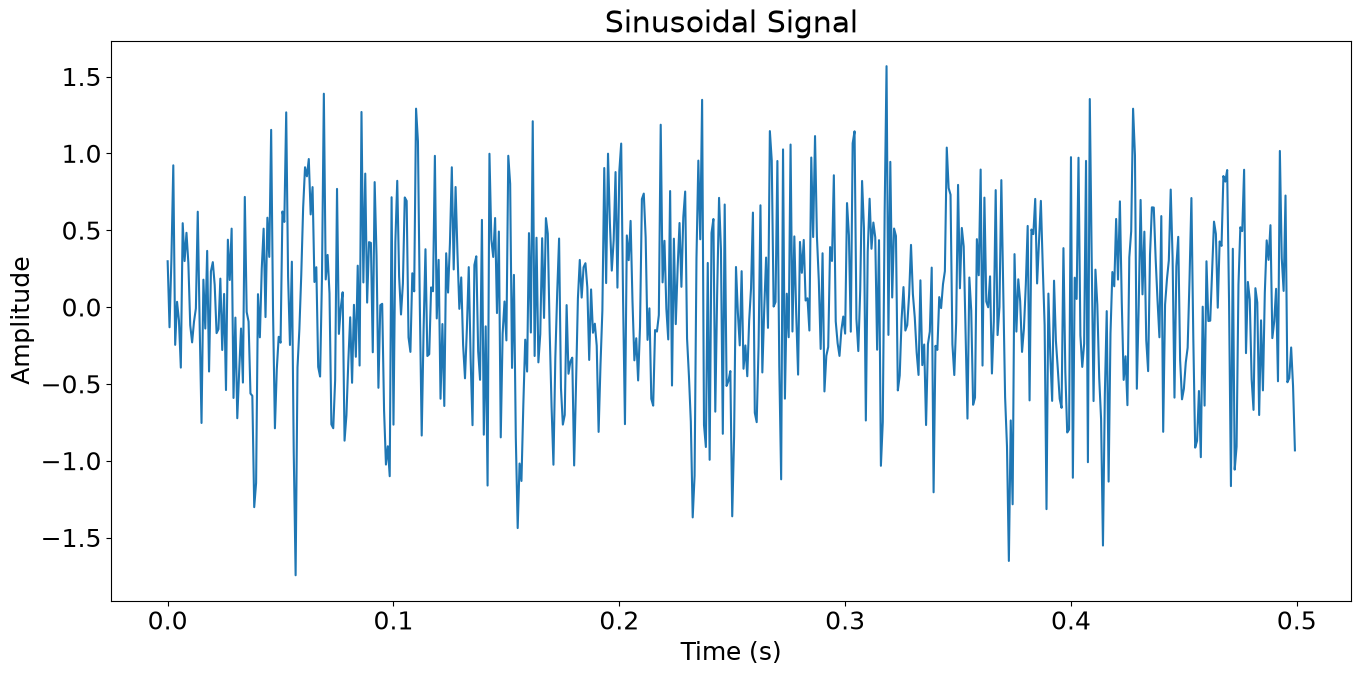
\includegraphics{time-domain.png}

\hypertarget{plot-the-magnitude-spectrum}{%
\subsubsection{Plot the magnitude
spectrum}\label{plot-the-magnitude-spectrum}}

Calculate the frequency axis for the spectrum, compute the FFT of the
generated signal \texttt{x} using \texttt{scipy.fftpack.fft}, and then
calculate the magnitude of the spectrum, then plot the magnitude
spectrum, showing the frequency components of the signal.

\begin{Shaded}
\begin{Highlighting}[]
\CommentTok{\# Generate freqeuncy axis}
\NormalTok{n }\OperatorTok{=}\NormalTok{ np.size(t)}
\CommentTok{\# We just need half of the samples in frequency domain since the signal is real{-}valued}
\NormalTok{fr }\OperatorTok{=}\NormalTok{ (fs}\OperatorTok{/}\DecValTok{2}\NormalTok{)}\OperatorTok{*}\NormalTok{np.linspace(}\DecValTok{0}\NormalTok{,}\DecValTok{1}\NormalTok{,}\BuiltInTok{int}\NormalTok{(n}\OperatorTok{/}\DecValTok{2}\NormalTok{))}
\CommentTok{\# Compute FFT of x}
\NormalTok{X }\OperatorTok{=}\NormalTok{ fft(x)}
\CommentTok{\# Magnitude of the FFT}
\NormalTok{X\_mag }\OperatorTok{=} \DecValTok{2}\OperatorTok{/}\NormalTok{n }\OperatorTok{*}\NormalTok{ np.}\BuiltInTok{abs}\NormalTok{(X[}\DecValTok{0}\NormalTok{:np.size(fr)])}

\NormalTok{plt.subplot(}\DecValTok{2}\NormalTok{,}\DecValTok{1}\NormalTok{,}\DecValTok{2}\NormalTok{)}
\NormalTok{plt.plot(fr, X\_mag)}
\NormalTok{plt.title(}\StringTok{\textquotesingle{}Magnitude of the Spectrum\textquotesingle{}}\NormalTok{)}
\NormalTok{plt.xlabel(}\StringTok{\textquotesingle{}Frequency (Hz)\textquotesingle{}}\NormalTok{)}
\NormalTok{plt.ylabel(}\StringTok{\textquotesingle{}Magnitude\textquotesingle{}}\NormalTok{)}
\NormalTok{plt.show()}
\end{Highlighting}
\end{Shaded}

\textbf{Output:}

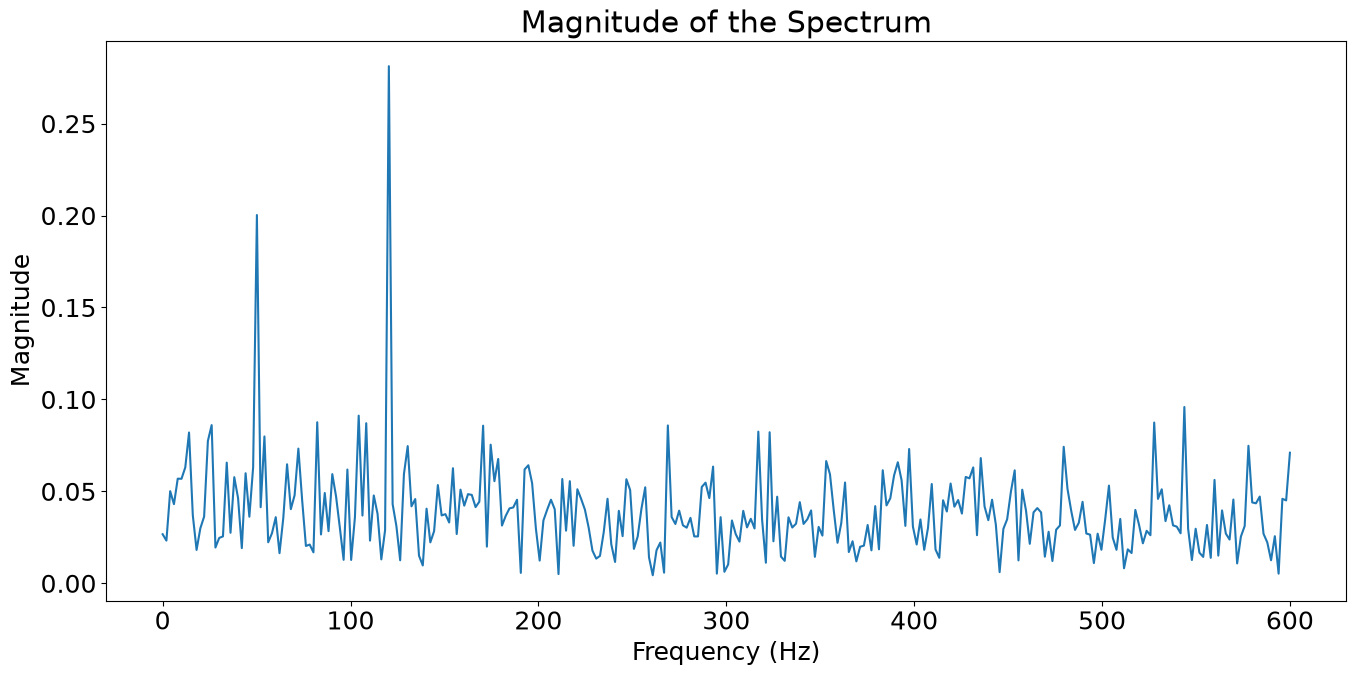
\includegraphics{magnitude-spectrum.png}
